% !TeX spellcheck = lt
\documentclass{VUMIFInfMagistrinis}
\usepackage{algorithmicx}
\usepackage{algorithm}
\usepackage{algpseudocode}
\usepackage{amsfonts}
\usepackage{amsmath}
\usepackage{bm}
\usepackage{color}
\usepackage{listings}
\usepackage{etoolbox}
\usepackage{graphicx}
\usepackage{hyperref}
\usepackage{setspace}

\newcommand{\argmax}{\operatornamewithlimits{argmax}}
% Titulinio aprašas
\university{Vilniaus universitetas}
\faculty{Matematikos ir informatikos fakultetas}
\department{Informatikos katedra}
\papertype{Magistro baigiamojo darbo literatūros apžvalga}
\title{Šalto starto problemos rekomendacinėse sistemose sprendimas naudojant socialinių tinklų duomenis}
\titleineng{Applying Social Network Data for Cold Start Problem in Recommender Systems}
\status{II kurso Informatikos studentas}
\author{Andrius Juškevičius}
% \secondauthor{Vardonis Pavardonis}   % Pridėti antrą autorių
\supervisor{lekt. Rimantas Kybartas}
\reviewer{prof. habil. dr. Antanas Žilinkskas}
\date{Vilnius – \the\year}

% Nustatymai
% \setmainfont{Palemonas}   % Pakeisti teksto šriftą į Palemonas (turi būti įdiegtas sistemoje)
\bibliography{bibliografija}

\begin{document}

\maketitle

%% Padėkų skyrius
% \sectionnonumnocontent{}
% \vspace{7cm}
% \begin{center}
%     Padėkos asmenims ir/ar organizacijoms
% \end{center}

\sectionnonumnocontent{Santrauka}
Žmonės priimdami sprendimus dažnai pasikliauja draugų ir pažįstamų rekomendacijomis. Vienas iš rekomendacinių sistemų (toliau - RS) metodų - bendradarbiavimo filtravimas (angl. Collaborative Filtering, toliau BF) nors ir naudoja metodą, imituojantį žmonių tarpusavio panašumą, ji negali identifikuoti, ką žmogus pažįsta, o ko ne. Socialinių tinklų duomenys užpildo šią spragą ir leidžia RS pateikti rekomendacijas atsižvelgiant ir į žmonių tarpusavio santykį. 
\newline
\indent
Šioje literatūros apžvalgoje pateikta rekomendacinių sistemų apžvalga, išnagrinėtas bendradarbiavimo filtravimo algoritmas, pristatytos duomenų retumo ir šalto starto problemos bei apžvelgtos socialinio tinklo duomenų taikymo galimybes sprendžiant šią problemą. Taip pat detaliai ištirti RS vertinimo matai ir kriterijai.
% Nurodomi iki 5 svarbiausių temos raktinių žodžių (terminų).
% Vienas terminas gali susidėti iš kelių žodžių.
\raktiniaizodziai{rekomendacinė sistema, bendradarbiavimo filtravimas, socialinis tinklas, šaltas startas}   

\tableofcontents

\section{Įvadas}
\linespread{1.5}
\selectfont
Rekomendacinės sistemos (toliau - RS) – programiniai įrankiai ir metodai, teikiantys rekomendacijas naudotojams. RS gali būti pagrindinis sistemos elementas,  arba pagalbinis įrankis platesnio taikymo sistemoje (elektroninėje parduotuvėje, filmų duomenų bazėje, kelionių agentūros sistemoje). Dėl plataus komercinio RS pritaikymo RS pastaruoju metu susilaukė daug tyrėjų dėmesio ir buvo stipriai patobulintos. 
\newline
\indent
Iš tiesų, dėl elementų gausos bet kurioje didelėje sistemoje, naudotojui yra sunku rasti tai, kas jam reikalinga arba galėtų jį sudominti. RS siekia pateikti naudotojui būtent jam skirtą rekomendaciją. Rekomendacijos suasmeninimas gali remtis arba elementu – siūlomas elementas, panašus į tus, kuriais naudotojas domėjosi anksčiau – arba naudotoju. Metodai, kuriuose naudotojas vaidina esminį vaidmenį, vadinami bendradarbiavimo filtravimo (angl. Collaborative-Filtering), toliau - BF, metodais. Jų esmė – rasti kitus naudotojus su panašiomis pirmenybėmis ir pasiūlyti naudotojui tai, kas patiko jiems. BF šiuo metu yra populiariausias RS metodas dėl savybių, kurios bus aprašytos toliau.
\newline
\indent
Bendradarbiavimas, tarpusavio sąveika ir dalinimasis informacija – pagrindinai naujos kartos tinklinių programų kartos, kitaip vadinamos Web 2.0, bruožai. Šiai kartai priklausančių socialinių tinklų atsiradimas atvėrė naujas galimybes RS tyrimų srityje. Papildžius tradicinėse RS naudojamus duomenis duomenimis iš socialinių tinklų apie naudotojų tarpusavio santykius, galima pagerinti rekomendacijų rezultatus ir bent iš dalies išspręsti kai kurias problemas, su kuriomis susiduriama tradicinėse RS. Be to, psichologiniai tyrimai rodo, kad žmonės labiau linkę pasitikėti, rekomendacijomis žmonių, kuriuos jie pažįsta. Tokios RS vadinamos pasitikėjimu sustiprintos RS (angl. Trust-enhanced recommender systems). Šios sistemos generuoja rekomendacijas, kurios remiasi informacija apie naudotojų profilius ir jų tarpusavio sąryšius. Minėtos, problemos, su kuriomis susidoroti padeda socialinių tinklų duomenys - šalto starto (angl. cold start) ir duomenų retumo problemos (angl. data sparcity). Šaltas startas - terminas, apibūdinantis situaciją, kai rekomendacinėje sistemoje atsiranda naujas elementas arba naudotojas. Tokiu atveju, dėl pradinės informacijos stygiaus sunku pateikti su jais susijusias rekomendacijas. Duomenų retumo problema panaši į šalto starto, tačiau apima visą duomenų rinkinį. Jos esmė - duomenų nepakankamumas sudaryti tinkamai rekomendacijai. Tipinėje sistemoje elementų aibė yra labai didelė (jų gali būti milijonai), tuo tarpu vieno naudotojo įvertintų elementų aibė yra labai maža (pvz., $10$). Tai reiškia, kad yra labai menkai tikėtina, kad du atsitiktiniai naudotojai turės bendrai įvertintų elementų, kitaip tariant, jie nėra palyginami.
\newline
\indent
Kitas aspektas į kurį būtina atsižvelgti modeliuojant RS yra jos atsparumas atakoms. Kalbant apie anksčiau minėtą pavyzdį apie retus duomenis galima pridurti, kad galima ataka, nutaikyta į konkretų naudotoją siekiant iškreipti jam pateikiamas rekomendacijas. Šioje apžvalgoje apie atakas bus tik užsiminta. 
\newline
\indent
Nors rekomendacinės sistemos kaip savarankiška tyrimų sritis buvo pradėtos tyrinėti dešimto dešimtmečio viduryje, užuomazgų galima rasti tokiose srityse kaip kognityvinis mokslas ir informacijos išgavimas. Šių dienų RS sritis taiko metodikas iš žmogaus ir kompiuterio sąveikos, informacijos išgavimo (angl. information retrieval) srities, taip pat naudoja duomenų išgavimo (angl. datamining) algoritmus.
\newline
\indent
Įvertinti RS tikslumą turint testinius duomenis ir atsižvelgus į jų struktūrą nėra sudėtinga. Vis dėlto, RS turi daug įvertinimo kriterijų, kuriuos galima įvertinti trijų rūšių eksperimentais – "offline", "online" ir naudotojų tyrimu. Būtent RS taikymo sritis nulemia, kurie kriterijai yra svarbiausi – gali būti, kad naudotojui visiškai nebus naudos iš to, kad RS rekomenduos teisingus dalykus, kuriuos naudotojas ir taip būtų sužinojęs. Vietoje to siekiama netikėto, bet naudotojui įdomaus rezultato. Skirtingi RS metodai turi skirtingas savybes – šie skirtumai plačiai bus apžvelgti kitame skyriuje. 
\newline
\indent
Šios literatūros apžvalgos tikslas - pateikti išsamią tyrimų apie pasitikėjimą rekomendacinėse sistemose ir šalto starto problemos analizę. Ši apžvalga turėtų būti pamatu siekiant magistro darbo tikslo - modifikuoti esamą bendradarbiavimo filtravimo metodą, taip, kad jis veiktų gerai tiek šalto starto scenarijaus atveju, tiek įprastoje aplinkoje (t.y. esant pakankamam reitingų skaičiui) ir apibrėžti rekomendacinės sistemos vertinimo kriterijus. Pasiūlius tokį metodą bus atlikti eksperimentai, tiriantys šių metodų efektyvumą ir įvairių parametrų bei skirtingų matų naudojimo įtaką pagal šiame darbe apibrėžtus vertinimo kriterijus. Iš šių tikslų išplaukiantys darbo rezultatai - teorinis metodo pagrindimas ir praktinis tyrimas.


\section{Bendradarbiavimo filtravimo (Collaborative-Filtering) metodas ir šalto starto problema}
\subsection{Rekomendacinių sistemų apžvalga ir bendradarbiavimo filtravimo metodas}
Visų pirma, suformuluokime RS sprendžiamą problemą formaliai taip, kaip tai padaryta \cite{2}. Vartotojų aibė pažymėkime $U$ ir elementų aibę $I$. Be to, pažymėkime $R$ aibę sistemoje turimų reitingų ir $S$ – aibę galimų reikšmių, kurias gali įgyti reitingas (pvz. $S=[1,5]$). Taip pat, tarkime, kad vienas reitingas $r_{ui}$ gali būti priskirtas vienam elementui $i \in I$ vieno naudotojo $u \in U$. Vartotojų poaibį, kuris yra įvertinęs elementą $i$, pažymėkime $U_i$. Analogiškai, $I_u$ pažymėkime aibę elementų, kuriuos yra įvertinęs naudotojas $u$. Daiktų, kuriuos yra įvertinę abu naudotojai $u$ ir $v$, aibę $I_u \and I_v$ pažymėkime $I_{uv}$. Analogiškai, $U_{ij}$ žymi aibę naudotojų, kurie yra įvertinę tiek elementą $i$, tiek $j$. Dvi dažniausiai sutinkamos problemos – geriausios ir geriausių $N$ rekomendacijos problema. Vienas būdų spręsti šias problemas yra įvertinti funkciją $f: U \times I -> S$, kuri nuspėja reitingą $f(u,i)$. Ši funkcija tada yra naudojama naudotojo $u_a$ rekomendacijai elemento $i^*$, kuriam įvertinamas reitingas turi didžiausią reikšmę $i^*= \arg \max \limits_{j \in \frac{I}{I_u}} f(u_a,j)$. 
RS galima modeliuoti dviem būdais:
\begin{itemize}
	\item Turiniu-pagrįstų metodų esmė – identifikuoti charakteristikas, kuriomis pasižymėjo elementai, kuriuos naudotojas įvertino palankiai praeityje ir tada naudotojui rekomenduoti kitus elementus su panašiomis charakteristikomis.
	\item Bendradarbiavimo-filtravimu pagrįsti metodai rekomenduoja elementus, kurie patiko naudotojams, turintiems panašias pirmenybes. BF metodai remiasi tik naudotojų suteiktais reitingais. Jie ieško panašumų tarp naudotojų pirmenybių ir tai lemia dvi geras savybes, kuriomis nepasižymi turiniu pagrįsti metodai
	\begin{itemize}
		\item įžvalgumas - siūlomi ne tik akivaizdūs pasiūlymai, bet ir netikėti (t.y. tokie, kokių naudotojas kitomis aplinkybėmis turbūt nerastų)
		\item pritaikymas skirtingose srityse, elementu pagrįstos rekomendacijos reikalauja specifinių srities parametrų duomenų (pvz., kiek tam tikras filmas yra komedija, kiek drama)
	\end{itemize}
\end{itemize}
Bendradarbiavimo filtravimo sąvoką pirmąsyk panaudojo Goldberg \cite{16}. Šį metodą  galima suskaidyti į dvi klases – atmintimi pagrįstų metodų ir modeliu pagrįstų metodų klasę. Atmintimi pagrįsti metodai dažniausiai remiasi  artimiausių kaimynų metodu ir naudoja duomenis tiesiogiai generuojant rekomendacijas. Modeliu pagrįstų metodų esmė – sudaryti nuspėjantį modelį, kurio apmokymui naudojami turimi duomenys. Keli verti dėmesio pavyzdžiai: Bajeso klasterizacija, latentinė semantinė analizė, Bolcmano mašinos, atraminių vektorių mašinos, tikrinių reikšmių išskaidymas (SVD). Šiems metodams prieš rekomendacijos generavimo žingsnį reikalingas tam tikras duomenų apdorojimas, kuris, esant dideliam duomenų kiekiui, gali kainuoti daug resursų. Dar vienas privalumas, kuriuo pasižymi atmintimi pagrįsti metodai yra tas,  kad tokiu būdu sugeneruotos rekomendacijos gali pateikti netikėtų pasiūlymų. Šioje apžvalgoje didžiausias dėmesys bus kreipiamas į turiniu pagrįstus metodus.
\newline
\indent
	Vartotoju pagrįsta reitingo prognozės esmė ta, kad parenkami artimiausi naudotojo kaimynai. Vartotojų tarpusavio artumas nustatomas naudojant panašumo metrikas, kurios bus aprašytos vėliau. Šią prognozę galima atlikti dvejopai:
	\begin{itemize}
		\item Taikant artimiausių kaimynų regresiją, reitingas įvertinamas skaičiuojant pasvertą artimiausių kaimynų vidurkį.
		\item Taikant artimiausių kaimynų klasifikaciją, elemento reitingas parenkamas toks pats, kokį jam yra suteikęs artimiausias naudotojo kaimynas
	\end{itemize}


Pagrindinis turiniu pagrįsto prieš naudotoju pagrįstą reitingo prognozavimo trūkumas yra tas, kad tokiu būdų sugeneruotos rekomendacijos yra nors ir tikslios, tačiau nelabai vertingos, nes rekomenduojami elementai pernelyg panašūs į tuos, kuriuos naudotojas jau žino. Šią problemą galima vertinti kaip pernelyg didelio pritaikymo (angl. over-specialization) problemą arba kaip įžvalgumo (angl. serendipity) stygių. Be to, naudotoju pagrįstas metodas yra paremtas realiu žinių perdavimo iš lūpų į lūpas modeliu, todėl, tikėtina, geriau modeliuoja žinių išgavimą.
\newline
\indent
Norėdami prognozuoti naudotojo $u$ reitingą elementui $i$, imame $k$ artimiausių kaimynų $N_i(u)$ ir ieškome jų vidurkio.
\begin{equation}
\hat{r}_{ui} = \frac{1}{N_i(u)}\sum \limits_{v \in N_i(u)} r_{vi}
\end{equation}
Ši formulė neatsižvelgia į naudotojų panašumą. Būtų neteisinga vertinti visus kaimynus vienodai, kai kai kurie yra panašūs į naudotoją $u$, o kai kurie visiškai nepanašūs. Panašumą įtraukiame kaip svorius.
	\begin{equation}\label{eq:1}
	\hat{r}_{ui} = \frac{\sum \limits_{v \in N_i(u)} w_{uv} r_{vi}}{\sum \limits_{v \in N_i(u)} |w_{uv}|}
	\end{equation}
Šioje formulėje naudojamas svertinis vidurkis yra dažniausiai praktikoje taikomas, paprastas ir tikslus būdas nustatyti prognozei, tačiau lieka klausimas - į kiek kaimynų reikia atsižvelgti. GroupLens sistemoje visi $U \setminus \{u\}$ laikomi kaimynais; kitose sistemose kaimynai parenkami pagal panašumo slenkstį. Kaimynų skaičiaus apribojimas leidžia įvertinti tikslesnes prognozes, nes taip sumažinamas kaimynų su maža koreliacija keliamas triukšmas. Dar kitas būdas - atsižvelgiant į dalykinę sritį parinkti konstantą. 


\subsection{Reitingų normalizavimas}
Kai kalbame apie bendradarbiavimo filtravimą, neišvengiamai kyla problema, kad naudotojų reitingų pasiskirstymas nėra vienodas – vienam naudotojui gali patikti beveik viskas, kitam beveik niekas. Tokiu atveju, būtų neteisinga teigti, kad abiejų tam tikram elementui suteiktas aukščiausias įvertinimas turi vienodą svorį.  Šios problemos sprendimui yra pasiūlyti du būdai.
\begin{itemize}
	\item Vidurkio centravimas. Jo esmė – nustatyti, ar reitingas yra teigiamas, ar neigiamas, lyginant jį su vidurkiu. Vartotoju paremtoje rekomendacijoje $h(r_{ui})$ reitingo $r_{ui}$ transformacija, gaunama iš reitingo $r_{ui}$ atimant naudotojo reitingų vidurkį $h(r_{ui}) = r_{ui} - \bar{r_u}$. Taikant šį metodą reitingo įvertis randamas taip: 
	\begin{equation}
	\hat{r}_{ui} = \bar{r}_u + \frac{\sum\limits_{v \in N_i(u)} w_{uv}(r_{vi} - \bar{r}_v)}{\sum\limits_{v \in N_i(u)} |w_{uv}|}
	\end{equation}
	Elementu paremtoje rekomendacijos atveju ši transformacija atliekama analogiškai.
\item	Z-reikšmių normalizacija, skirtingai nei vidurkio centravimas, atsižvelgia ir į reitingų pasiskirstymą. Reitingo transformacija randama taip: $h(r_{ui}) = \frac{r_ui-\bar{r}_u}{\sigma_u}$ ir naudotoju paremto reitingo prognozė tada yra 
\begin{equation}
\hat{r}_{ui} = \bar{r}_u + \sigma_u \frac{\sum\limits_{v \in N_i(u)} w_{uv (r_{vi} - \bar{r}_v)/ \sigma_v}}{\sum\limits_{v \in N_i(u)} |w_{uv}|}
\end{equation}
				
\end{itemize}
\subsection{Vartotojų panašumo apskaičiavimas}
\subsubsection{Pyrsono koreliacija}

	Pyrsono koreliacija skirta statistinės koreliacijos radimui:
	\begin{equation}
	s(u,v) = \frac{\sum \limits_{i\in I_u \cap I_v }(r_{u,i}-\bar{r}_u)(r_{v,i}-\bar{r}_v)}{\sqrt{\sum\limits_{i \in I_u \cap I_v }(r_{u,i} - \bar{r}_u)^2}\sqrt{\sum\limits_{i \in I_u \cap I_v }(r_{v,i} - \bar{r}_v)^2}}
	\end{equation}
	Šis metodas susiduria su sunkumais, kai reikia paskaičiuoti panašumą tarp naudotojų, kurie bendrai yra įvertinę mažai elementų. Galima išeitis - nustatyti slenkstį, nuo kurio koreliacija būtų baudžiama. Taigi panašumą $s(u,v)$ tokiu atveju reiktų dauginti iš $min{|I_u \cap I_v|, 1}$.
	\subsubsection{Apribota Pyrsono koreliacija}
	Kai kalbame apie šį metodą, pereiname nuo tolydinio prie kategorinio parametrų vertinimo. Be to, atsižvelgiama į nuokrypį ne nuo vidurkio, o nuo abejingumo įverčio. Jeigu turime reitingų skalę nuo 1 iki 7, tada 4 reiškia abejingumą. Pažymėkime $r_x = 4$. Tada Shardanand ir Maes pasiūlyta apribota Pyrsono koreliacija randama taip
	\begin{equation}
	s(u,v) = \frac{\sum \limits_{i\in I_u \cap I_v }(r_{u,i}-r_z)(r_{v,i}-r_z)}{\sqrt{\sum\limits_{i \in I_u \cap I_v }(r_{u,i} - r_z)^2}\sqrt{\sum\limits_{i \in I_u \cap I_v }(r_{v,i} - r_z)^2}}
	\end{equation}
\subsubsection{Spearmano rango koreliacija}
	Spearmano rango koreliacija panaši į Pyrsono koreliaciją, vienintelis skirtumas toks, kad skaičiuojant Spearmano koreliaciją, naudotojo reitingai yra surūšiuojami didėjimo tvarka, jiems priskiriami rangai - mažiausią reikšmę turintis reitingas gauna reikšmę 1. Tokiu būdu išvengiama reitingų normalizavimo problemos. Šis metodas veikia ne itin gerai, kai yra mažas galimų reikšmių skaičius, be to skaičiavimo požiūriu reikalaujantis daugiau resursų dėl surūšiavimo žingsnio.
\subsubsection{Kosinuso panašumas}
	Šis metodas skiriasi nuo ankstesnių tuo, kad yra į problemą žiūrima ne iš statistinio, o iš tiesinės algebros požiūrio taško. Vartotojai atvaizduojami kaip $|I|$ dimensijų turintys vektoriai, o panašumas apskaičiuojamas, kaip kosinuso atstumas tarp dviejų reitingo vektorių. Jis randamas sudauginant šiuos vektorius ir padalinant iš $L2$ (Euklido) normų sandaugos:
	\begin{equation}
	s(u,v) = \frac{\boldsymbol{r}_u \cdot \boldsymbol{r}_v}{||\boldsymbol{r}_u||_2 ||\boldsymbol{r}_v||_2}
	\end{equation}
\subsubsection{Euristinis PIP panašumo matas}
Euristinis panašumo matas pasiūlytas \cite{7} kreipia dėmesį į šalto starto problemą. Dažniausias šalto starto problemos sprendimo būdas - naudoti hibridines RS, kurios naujiems naudotojams rekomendacijas pateikia naudodamos turinio informaciją ir tik surinkus pakankamai duomenų apie naudotoją, įjungiamas BF režimas. Ši panašumo metrika atsižvelgia į šalto starto problemą panašumą apskaičiuodama remdamasi trimis faktoriais - panašumu, poveikiu, populiarumu.
	\begin{equation}
	\boldmath{SIM}(u_i, u_j)= \sum \limits_{k \in C, j}\boldmath{PIP}(r_{i,k}, r_{j,k})
	\end{equation}
	čia $r_{ik}$ ir $r_{jk}$ reitingai elementui $k$ nuo naudotojų $i$ ir $j$ atitinkamai, $PIP(r_{ik}, r_{jk})$ - $PIP$ reikšmė reitingams $r_{ik}$ ir $r_{jk}$
	\begin{equation}
	PIP(r_1,r_2) = Proximity(r_1,r_2) \times Impact(r_1,r_2) \times Popularity(r_1,r_2)
	\end{equation}
	Detalesnis aprašymas, kaip randamos šios reikšmės yra \cite{7}.
\subsubsection{Panašumas su svoriais}
 Said \cite{13} pastebėjo, kad dažniausiai naudojami panašumo matai (Pyrsono koreliacija, kosinuso panašumas) turi tokį trūkumą, kad jie neatsižvelgia į bendrai įvertintų elementų populiarumą - bendrai daugelio naudotojų įvertinti elementai vertinamam panašumui turėtų daryti mažesnę įtaką negu retai vertinami. Šį trūkumą siūloma spręsti panašumo matuose įvedant populiarumo svorius.
\newline
\indent
Tokiu būdu randama Pyrsono koreliacija atrodytų taip:
\begin{equation}
	s_w(u,v) = \frac{\sum \limits_{i\in I_u \cap I_v }w_i(r_{u,i}-\bar{r}_u)(r_{v,i}-\bar{r}_v)}{\sqrt{\sum\limits_{i \in I_u \cap I_v }w_i(r_{u,i} - \bar{r}_u)^2}\sqrt{\sum\limits_{i \in I_u \cap I_v }w_i(r_{v,i} - \bar{r}_v)^2}}
\end{equation}
ir kosinuso panašumas:
	\begin{equation}
	s_w(u,v) = \frac{\sum \limits_{i\in I_u \cap I_v} w_i \cdot r_{u,i} \cdot r_{v,i}}{\sqrt{\sum\limits_{i \in I_u} w_i \cdot r_{u,i}^2}\sqrt{\sum\limits_{i \in I_v} w_i \cdot r_{v,i}^2}}
	\end{equation}
o svoriai $w_i$ gali randami būti randami tokiais būdais:
	\begin{equation}
	w_i^{inf} = \log \frac{|U|}{|U_i|}
	\end{equation}
	\begin{equation}
	w_i^{lin} = 1 - \frac{|U_i|}{|R|}
	\end{equation}
Čia $|U|$ - naudotojų skaičius, $|U_i|$ - naudotojų, įvertinusių elementą $i$ skaičius, $|R|$ reitingų skaičius.
\newline
\indent
Šaltinyje \cite{13} parodyta, kad šis metodas geriausiai veikia vartotojams "po šalto starto" (angl. post cold start users), kai reitingų skaičius yra tarp 20 ir 80, kitiems rėžiams rezultatai buvo labai panašūs į tuos, kurie buvo gauti naudojant Pyrsono koreliaciją be svorių.  
\section{Pasitikėjimu pagrįstos rekomendacinės sistemos}
\subsection{Pasitikėjimo apžvalga}
Įžangoje buvo paminėta, kad žmonės labiau linkę pasitikėti pažįstamų pateiktomis rekomendacijomis. Susieję šį teiginį su faktu, kad socialiniai tinklai vis stipriau integruojasi į daugumos žmonių gyvenimą, gauname prielaidą pasitikėjimu sustiprintų rekomendacinių sistemų atsiradimui. Veikiantis pavyzdys - Goelbeck FilmTrust - socialinis tinklas susietas su filmų reitingavimo sistema, kurioje naudotojai yra prašomi įvertinti jų draugų skonį skalėje nuo 1 iki 10.
\newline
\indent
Tokiose sistemose naudotojas gauna rekomendaciją elemento, turinčio aukštą įvertinimą naudotojo WOT - pasitikėjimo tinkle (angl. web of trust). Pagrindiniai tokių sistemų įrankiai yra agregavimo (angl. aggregation) ir propagavimo (angl. propagation) operatoriai. Propagavimo operatorius taiko pasitikėjimo tranzityvumo prielaidą - jeigu naudotojas $a$ pasitiki naudotoju $b$, o $b$ pasitiki $c$, tai $a$ pasitiki $b$. Agregavimo operatorius apjungia kelis pasitikėjimo įverčius į vieną.
\newline
\indent
Tikimybiniu požiūriu pasitikėjimas gali įgyti tik dvi reikšmes - arba kitu naudotoju galima pasitikėti (su tikimybe $p$), arba ne. Nors šia kryptimi buvo atlikta nemažai tyrimų, kur kas labiau įtikinantis yra laipsniškas požiūris, teigiantis, kad ne viskas yra tik juoda arba balta. Šiuo požiūriu pasitikėjimas nėra vertinamas kaip tikimybė, didesnė reikšmė tiesiog reiškia didesnį pasitikėjimą. Čia galima pastebėti ir analogiją su realiu gyvenimu - vienais žmonėmis pasitikime daugiau, kitais mažiau. 
\newline
\indent
Nors pasitikėjimas, kaip nagrinėjamas reiškinys, RS kontekste įdomus palyginti neseniai,  kitose srityse atlikta nemažai tyrimų. Verti paminėjimo tyrimai psichologijoje, sociologijoje, komunikacijoje, darbo rinkos srityse. XXI amžiuje išpopuliarėjus internetui ir socialiniams tinklams atsirado aibė reikalingų duomenų tokiems tyrimams. Golbeck savo disertacijoje \cite{10} pateikė kriterijus, kuriuos turi tenkinti socialinis tinklas:
\begin{itemize}
	\item yra pasiekiamas per internetą naudojant interneto naršyklę
	\item jame naudotojai turi patys nustatyti tarpusavio ryšį
	\item jis turi būti skirtas tiems ryšiams palaikyti
	\item jame santykiai gali būti peržiūrimi ir naršomi
\end{itemize} 

\subsection{Pasitikėjimo apskaičiavimas}
Pasitikėjimo tinkle dauguma naudotojų vienas kito nepažįsta. Nepaisant to, reikia nustatyti sąryšius tarp jų. Tam yra naudojamos pasitikėjimo metrikos, kurios remdamosi naudotojų santykiais nustato, kiek vienas naudotojas pasitiki kitu. Pasitikėjimo metrikos skyla į dvi klases.
\begin{itemize}
	\item Lokalios metrikos įvertina pasitikėjimą kiekvienam naudotojui individualiai - dėl to jos gali būti tikslesnės ir reikalauja daugiau skaičiavimo resursų. Toliau bus pristatyti lokalių metrikų pavyzdžiai - TidalTrust, MoleTrust.
	\item Globalios metrikos įvertina bendrą elemento reitingą visoje pasitikėjimo sistemoje. Apie jas toliau kalbama nebus, žymiausias pavyzdys - PageRank algoritmas naudojamas Google paieškos sistemoje.
\end{itemize}
Kaip minėta, pasitikėjimo skaičiavimui svarbi tranzityvumo prielaida, tačiau, ji teisinga tik tame pačiame kontekste - jeigu $a$ pasitiki $b$ kai kalbama apie automobilius, o $b$ pasitiki $c$ sodininkystės klausimais, nieko negalėsime pasakyti apie $a$ pasitikėjimą $c$ kompiuterijos žiniomis.
\newline
Toliau bus pristatyti propagavimo operatoriai. Kol kas nesigiliname į tai, kaip gaunami pasitikėjimo įverčiai, laikome juos duotais.
\indent
\begin{itemize}
	\item Vienas dažniausiai naudojamų propagavimo operatorių (ypač, kai kalbame apie tikimybinį požiūrį) yra daugyba. Pavyzdžiui, $a$ pasitiki $b$ $0.8$, o $b$ pasitiki $c$ $0.5$, tada $a$ pasitiki $c$ $0.8 \times 0.5 = 0.4$. 
	\item Kitas operatorius - silpniausios grandies. Anksčiau pateikto pavyzdžio atveju $a$ pasitikėjimas $c$ būtų lygus $0.5$. 
	\item Konjunkcijos operatorius - $max(t_1+t_2-1)$ ankstesniame pavyzdyje grąžintų $0.3$ $A$ pasitikėjimą $C$.
\end{itemize}
Žinoma, ne visi propagavimo keliai yra vienodo ilgio. Intuityviai aišku, kad svarbesni yra trumpesni keliai ir kuo ilgesnis kelias - tuo mažiau informacijos jis suteikia. Ši problema nesunkiai sprendžiama - vieni autoriai naudoją skleidimo faktorių \cite{17}, kiti atsižvelgia tik į trumpiausią kelią.

\begin{figure}[ht!]
	\centering
	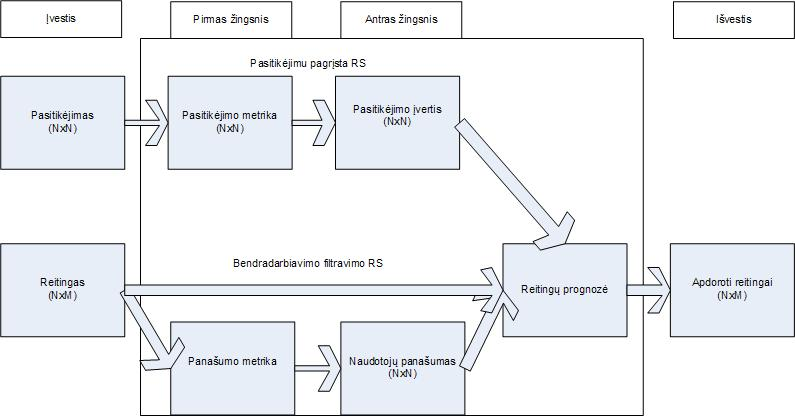
\includegraphics[width=160mm]{Drawing1.jpg}
	\caption{Pasitikėjimu pagrįstos ir paprastos bendradarbiavimo filtravimo RS architektūros palyginimas \label{5_vs_BF}}
\end{figure}

\ref{5_vs_BF} pavaizduotoje schemoje pavaizduotas dviejų metodų palyginimas. Abu metodai remiasi panašiomis prielaidomis, iš esmės skiriasi svorių $|w_{uv}|$ formulėje \eqref{eq:1} radimo būdai. Pasitikėjimu pagrįstoje RS panašumas tarp naudotojų randamas taikant pasitikėjimo metrikas, o ne įvertinant panašumą, kaip tai daroma tradicinėse BF RS. Toliau pristatomos pasitikėjimo metrikos.
\subsubsection{TidalTrust}
 Ši formulė yra esminė Golbeck rekomendacijos algoritme. Algoritmo autoriai šią formulę išvedė atlikdami eilę eksperimentų, kurių metu jie ignoruodami tiesioginį naudotojo $a$ pasitikėjimą naudotoju $c$ tyrinėjo kelius, jungiančius šiuos du naudotojus. Lygindami taikant išskaidymą (angl. propagation) gautus įverčius su tikromis pasitikėjimo reikšmėmis jie pastebėjo, kad: 
\begin{itemize}
	\item trumpesni išskaidymo keliai leidžia apskaičiuoti tikslesnius pasitikėjimo įverčius
	\item keliai su didesnėmis pasitikėjimo reikšmėmis taip pat leidžia apskaičiuoti didesnius pasitikėjimo įverčius
\end{itemize}
Remiantis pirmu pastebėjimu buvo sugalvota, kad reikia apriboti kelio ilgį tarp naudotojų. Nustačius fiksuotą kelio ilgį gali atsitikti taip, kad tik maža dalis naudotojų gali būti pasiekiama. Dėl šios priežasties nustatytas kintamas galimas kelio ilgis - ilgiausias kelias, reikalingas sujungti tikslinį naudotoją su naudotoju, įvertinusiu elementą $i$.
\newline
\indent
Atsižvelgdami į kitą pastebėjimą (apie didesnes pasitikėjimo reikšmes vedančias prie tikslesnių įverčių) autoriai siūlo apriboti informaciją taip, kad ji būtų gaunama tik iš patikimiausių naudotojų. Tačiau čia vėl reikia pastebėti, kad skirtingi žmones turi skirtingas pasitikėjimo skales - vienas gali pasitikėti visais, kitas - beveik niekuo. Be to, dažnai būna taip, kad mažai kelių turi tokią pačią pasitikėjimo reikšmę. Dėl šių priežasčių Golbeck nusprendė įvesti reikšmę, atspindinčią kelio stiprumą (t.y. mažiausią pasitikėjimo reitingą kelyje) ir apskaičiuoti maksimalų kelio stiprumą $max$ (iš visų kelių, vedančių prie elementą vertinusių naudotojų), kuris po to naudojamas kaip slenkstis dalyvavimui algoritme.
\begin{equation}\label{eq:TIDAL5}
t_{a,u} = \frac{\sum\limits_{v \in WOT^{+}(a)}t_{a,v}t_{v,u}}{\sum\limits_{v \in WOT^{+}(a)}t_{a,v}}
\end{equation}
\eqref{eq:TIDAL5} pateikta TidalTrust formulė. Joje $WOT^{+}(a)$ atspindi naudotojų aibę, kuriems naudotojo $a$ pasitikėjimo jais reikšmė viršija slenkstį $max$.
\newline
\indent
Šis algoritmas yra rekursinis - $t_{a,u}$ rekursiškai skaičiuojamas, kaip svertinis pasitikėjimo reikšmių $t_{v,u}$ vidurkis. Šis algoritmas priklauso laipsniškų pasitikėjimo algoritmų klasei ir yra lokalios pasitikėjimo metrikos pavyzdys.
\newline
\indent
Golbeck parodė, kad pasitikėjimu pagrįstas svertinis vidurkis kartu su TidalTrust nebūtinai visada yra pranašesnis už BF, tačiau duoda žymiai geresnius įverčius naudotojams, kurie nesutinka su vidutiniu elemento $i$ reitingu.
\subsubsection{MoleTrust}
\begin{equation}\label{eq:MOLE5}
p_{a,i} = \bar{r_a}+\frac{\sum\limits_{u \in R^T}t_{a,u}(r_{u,i}-\bar{r_u})}{\sum\limits_{u \in R^T} t_{a,u}}
\end{equation}
\eqref{eq:MOLE5} formulė - Massa \cite{11} pasiūlyto rekomendacijų algoritmo pagrindas. Ši metrika susideda iš dviejų žingsnių:
\begin{itemize}
	\item pirmame žingsnyje pašalinami pasitikėjimo tinkle esantys ciklai
	\item antrame žingsnyje atliekamas pasitikėjimo apskaičiavimas
\end{itemize}
Ciklų pašalinimo esmė ta, kad kiekvienas naudotojas tinkle būtų aplankytas tik kartą siekiant didesnio efektyvumo vykdant išskaidymą (angl. propagation).
Ciklų pašalinimu transformuojame pradinį tinklą į kryptinį beciklį grafą. Tuomet pasitikėjimo prognozę $t_a,u$ galime rasti atlikdami paprastą grafo apėjimą - visų pirma, randamas pasitikėjimas naudotojais, iki kurių atstumas lygus 1, tada pasitikėjimas tais, iki kurių atstumas 2 ir taip toliau. Verta pastebėti, kad pasitikėjimo naudotoju, esančių atstumu $x$ priklauso nuo anksčiau apskaičiuotų pasitikėjimo reikšmių naudotojams esantiems atstumu $x-1$.
\newline
\indent
Pasitikėjimas naudotojais, esančiais atstumu didesniu nei $1$ skaičiuojamas panašiu būdu, kaip \eqref{eq:TIDAL5}. TidalTrust naudotojas yra pridedamas prie $WOT^+(a)$ tada ir tik tada, jeigu jis yra trumpiausiame kelyje nuo naudotojo $a$ iki elemento $i$. MoleTrust atveju $WOT^+(a)$ apima visus naudotojus, kurie įvertino tam tikrą elementą ir gali būti pasiekti pasitikėjimo tinklu per ne daugiau kaip $d$ žingsnių. Parametras $d$ vadinamas išskaidymo horizontu. Kitas MoleTrust parametras - pasitikėjimo slenkstis, kuris TidalTrust algoritme buvo apibrėžtas kaip dinamiška $max$ reikšmė. MoleTrust pasitikėjimo slenkstis - fiksuotas dydis. 
\newline
\indent
MoleTrust taip pat priklauso laipsniškų lokalių pasitikėjimo metrikų klasei. Algoritmo autoriai eksperimentu parodė, kad MoleTrust randa geresnius pasitikėjimo įverčius nei globalios pasitikėjimo metrikos, tokios kaip naudojamos pavyzdžiui eBay, ypač kai kalba eina apie kontraversiškus naudotojus, kuriuos dalis vertina kaip labai patikimus, o kita dalis - labai nepatikimus. Autoriai taip pat parodė, kad šis algoritmas išgauna tikslesnes prognozes naujiems naudotojams.
\subsubsection{Pasitikėjimu pagrįstas svoris}
Šis metodas pristatytas \cite{12} naudoja vartotojo ir tiekėjo sąvokas. Reitingo prognozė skaičiuojama panašiai kaip \eqref{eq:1}:
\begin{equation}
c(i) = \bar{c}+\frac{\sum \limits_{p \in P(i)} (p(i) - \bar{p}) w(c,p,i)}{\sum \limits_{p \in P(i)} |w(c,p,i)|}
\end{equation}
$w(c,p,i)$ yra panašumo ir pasitikėjimo harmoninis vidurkis 
\begin{equation}
w(c,p,i) = \frac{2(sim(c,p))(trust(p,i))}{sim(c,p)+trust(p,i)}
\end{equation}
čia $c$ - vartotojas (angl. consumer), $p$ - gamintojas (angl. producer), $i$ -elementas, $sim(c, p)$ - panašumas tarp vartotojo ir gamintojo. $trust(p,i)$ matuoja kiek $c$ gali pasitikėti $p$ elemento $i$ vertinimu ir yra randamas taip:
\begin{equation}
trust(p,i)=\frac{|\{(c_k, i_k) \in CorrectSet(p): i_k = i\}|}{|\{(c_k,i_k) \in RecSet(p): i_k=i\}|}
\end{equation}
Šis reiškinys rodo, kokia dalis naudotojo $p$ rekomendacijų būna teisinga. Taip randamas pasitikėjimas vadinamas profilio lygio pasitikėjimu (angl. profile-level trust).
\section{RS vertinimas}
\subsection{RS vertinimo metodai}
Dažniausiai RS vertinimui naudojamas metodas vadinama vidutine absoliučia klaida (angl. Mean Absolute Error, trumpinama MAE) pagrįsta principu "išimk vieną" (angl. leave-one-out). 
\begin{equation}
MAE = \sqrt{\frac{1}{|T|}\sum\limits_{(u,i)\in T} |\hat{r}_{ui} - r_{ui}|}
\end{equation}
Šio metodo esmė - iš duomenų rinkinio išimti vieną reitingą ir atlikti jo prognozę. Prognozė tada lyginama su tikru reitingu ir taip randama prognozės klaida. Šis metodas tokį trūkumą, kad kiekvieną klaidą ieško vienodu būdu. Pavyzdys, iliustruojantis, kodėl tai yra negerai toks: tarkime, turime $101$ naudotoją $1$ yra įvertinęs $300$ elementų, o $100$ - po $3$. Tokiu atveju aptariamas duomenų rinkinys turi $600$ reitingų. Testuodami RS "išimk vieną" principu, slėptume iš eilės visus reitingus ir bandytume juos nuspėti. Bėda ta, kad RS kur kas geriau veikia naudotojams, turintiems daug reitingų ir prasčiau naujiems (arba nelinkusiems reitinguoti) naudotojams. MAE atveju vienas daug reitingų suteikęs naudotojas turi tokį patį svorį, kaip likę $300$. Akivaizdu, kad taip iškreipiama realybė - $300$ nepatenkintų naudotojų prieš $1$ patenkintą reiškia, kad sistema nėra tokia gera. Tam, kad išspręsti šią problemą buvo pasiūlytas patobulintas metodas - vidutinė absoliuti naudotojo klaida (angl. MAUE - Mean Average User Error). Jo esmė paprasta - randame MAE kiekvienam naudotojui ir tada randame visų naudotojų MAE vidurkį. Tokiu būdų, kiekvienas naudotojas turi lygų svorį skaičiuojant vidutinę klaidą.
\newline
\indent
Alternatyvus MAE metodas yra vidutinės kvadratinės klaidos šaknis (angl. RMSE- Root Mean Squared Error):
\begin{equation}
RMSE = \sqrt{\frac{1}{|T|}\sum\limits_{(u,i)\in T} (\hat{r}_{ui} - r_{ui})^2}
\end{equation}
RMSE palyginus su MAE stipriau baudžia už dideles klaidas. Pavyzdžiui, duomenų aibėje su keturiais paslėptais reitingais RMSE geriau vertintų sistemą, kurios klaida lygi $2$ trims reitingams ir $0$ vienam reitingui, negu sistemą, kuri klysta $3$ vienai reikšmei ir neklysta likusioms trims. MAE geriau vertintų antrą sistemą.
\newline
\indent
Kitas svarbus RS vertinimo matas yra - padengimas (angl. coverage). Herlocker RS vertinimo metodų apžvalgoje pabrėžia, kaip svarbu yra žiūrėti ne tik į tikslumą, bet ir į padengimą bei nurodo į kelis darbus tyrusius šią sritį. Padengimas - sąvoka skirta apibūdinti keliems skirtingiems aspektams:
\begin{itemize}
	\item Elementų erdvės padengimas (angl. item space coverage) apibūdina, kokią dalį visų RS esančių elementų RS gali rekomenduoti. Tai dar vadinama katalogo padengimu. Paprasčiausias būdas apskaičiuoti šį rodiklį - rasti procentą elementų, kurie gali būti rekomenduoti. Kitas katalogo padengimo matas - pasiūlymų įvairumas - matuoja kaip nevienodai pasirenkami skirtingi elementai, kai naudojama tam tikra RS. Šį matą galima apskaičiuoti keliais būdais:
	\begin{itemize}
	\item jeigu kiekvienas elementas $i$ sudaro $p(i)$ dalį naudotojo pasirinkimų, galime apskaičiuoti Gini indeksą:
	\begin{equation}
	G=\frac{1}{n-1} \sum\limits_{j=1}^{n} (2j-n-1)p(i_j)
	\end{equation}
	Kai visi elementai pasirenkami vienodai dažnai indekso reikšmė lygi $0$, kai visada pasirenkamas vienas elementas - $1$.
	\item Shannon'o entropija lygi 0, kai tas pasirenkamas tas pats elementas ir $\log n$ kai visi elementai pasirenkami vienodai dažnai
	\begin{equation}
	H= - \sum \limits_{i=1}^n p(i) \log p(i)
	\end{equation}
	\end{itemize}
	\item Naudotojų erdvės padengimas (angl. user space coverage) - terminas, nusakantis, kuriai daliai naudotojų RS gali sugeneruoti rekomendaciją. Kartais RS negali nieko rekomenduoti tam tikram naudotojui dėl mažo pasitikėjimo prognozės tikslumu. Toks padengimas gali būti įvertintas matuojant naudotojo profilio turiningumą, reikalingą, kad jam būtų sugeneruota rekomendacija. BF atveju tai galėtų būti mažiausias reitingų skaičius, kuri naudotojas privalo suteikti tam, kad gautų rekomendaciją.
\end{itemize}
Šaltas startas gali būti laikomas padengimo problemos dalimi. Norėdami spręsti šalto starto problemą, galima nustatyti slenkstį, apibrėžiantį, kada elementai yra "šalti". Pavyzdžiui, galima laikyti elementą "šaltu", jeigu jis neturi nė vieno reitingo arba, jeigu elementas sistemoje yra trumpiau nei nustatytą laiko tarpą.
\newline
\indent
Gali būti, kad sistema geriau rekomenduos "šaltus" elementus, "karštų" elementų rekomendacijos kaina. Tai gali būti trokštamas RS bruožas, ypač jeigu yra svarbios naujoviškumo ir įžvalgumo savybės.
\subsection{RS vertinimo aspektai}
\cite{3} pristatyti kelios RS savybės - prognozės tikslumas, padengimas, pasitikėjimas, patikimumas, naujoviškumas, įžvalgumas, įvairumas, naudingumas, rizika, atsparumas atakoms, privatumas, pritaikomumas, praplečiamumas. Visų jų šioje apžvalgoje dėl gausos pristatyti neįmanoma, todėl toliau bus pristatytos tik įdomiausios šio darbo kontekste - buvo paminėtos anksčiau.
\subsubsection{Patikimumas}
Patikimumą (angl. confidence) geriausia apibūdinti pavyzdžiu. Jeigu sistema pasiūlo naudotojui du elementus su vienodais prognozuojamais reitingais, tačiau vienos rekomendacijos patikimumas yra mažesnis nei kitos, tai naudotojui gali būti pravartu ją atidžiau patikrinti - perskaityt aprašymą ar pan. 
\subsubsection{Pasitikėjimas}
Pasitikėjimas (angl. trust) skiriasi nuo patikimumo tuo, kad pasitikėjimas matuoja sistemos pasitikėjimą reitingais, o pasitikėjimas šiuo atveju nurodo į naudotojo santykį su reitingais. Sistema, siekdama padidinti pasitikėjimą gali pasiūlyti kelis elementus, kuriuos naudotojas jau žino ir mėgsta. Kitas būdas, kaip padidinti pasitikėjimą - paaiškinti naudotojui, kodėl jam siūlomas vienas ar kitas elementas.
\subsubsection{Naujoviškumas}
Naujoviškos rekomendacijos naudotojams siūlo elementus, apie kuriuos jie nežinojo anksčiau. Paprasčiausias būdas padidinti rekomendacijų naujoviškumą - eliminuoti iš galimų elementų aibės jau vertintus ir peržiūrėtus elementus, tačiau šis metodas nepakankamas, jeigu norime iš rekomendacijų pašalinti visus elementus, apie kuriuos naudotojas jau žino.
\newline
\indent
Norint ištirti RS naujoviškumą paprasčiausia tai padaryti "on-line" eksperimentu. Vis dėlto, tai gali būti brangu, todėl buvo sugalvotas ir "off-line" eksperimento metodas. Metodo esmė tokia: nuo pasirinkto laiko taško reitingai yra paslepiami. Rekomenduojant sistema gautų taškų už kiekvieną iš tiesų įvertintą elementą ir baudžiama už kiekvieną elementą, kuris buvo rekomenduotas iki pasirinkto laiko taško.
\newline
\indent
Tarkime, norime įvertinti rekomendacijų naujoviškumą. Darydami prielaidą, kad naudotojai įvertina elementus, po to kai jais pasinaudoja, padaliname reitingus. Kiekvienam testuojamam naudotojui atsitiktinai parenkame laiko tašką, nuo kurio reitingai paslepiami. Tyrimai parodė, kad žmonės labiau linkę įvertinti elementus, kurie jiems arba labai patiko, arba labai nepatiko. Taigi, slepiame reitingus esančius prieš nukirpimo tašką su tikimybe $1-\frac{|r-3|}{2}$, kur $r \in \{1,2,3,4,5\}$ galimų elemento reitingų aibė, o $3$ yra neutralus reitingas. Siekiama, vengti paslėptų elementų prognozavimo, nes naudotojas apie juos jau žino. Tada kiekvienam naudotojui sugeneruojamos $5$ rekomendacijos ir skaičiuojamas jų tikslumas atmetant rekomendacijas elementų, rekomenduotų iki pasirinkto laiko taško. RS su didesniu tikslumu laikomos pranašesnėmis.
\subsubsection{Įžvalgumas}
Įžvalgumu matuojama, kiek stebinančios yra sėkmingos rekomendacijos. Pavyzdžiui, kalbant apie filmų RS, jeigu naudotojas įvertino daug filmų su tam tikru aktoriumi, pasiūlytas filmas su tuo pačiu aktoriumi gali būti naujoviškas, tačiau vargu ar galėsime šią rekomendaciją vadinti netikėta. Iš kitos pusės, atsitiktinės rekomendacijos gali būti labai stebinančios, tačiau reikia išlaikyti ir tikslumą.
\newline
\indent
Vienas būdų suprojektuoti sistemą, taip, kad jos pasiūlymai būtų įžvalgesni yra toks - nustačius atstumo matą tarp elementų, remiantis jų turiniu, sėkmingą rekomendaciją galime vertinti labiau, jeigu ji yra "toliau" nuo jau anksčiau teigiamai įvertintų elementų. Pavyzdžiui, turime knygų RS ir norime naudotojui rekomenduoti knygas autorių, kurių jis nežino. Tuomet turime sukonstruoti metriką tarp knygos $b$ ir anksčiau perskaitytų knygų aibės $B$. Tarkime $c_{B,w}$ - autoriaus $w$ knygų skaičius aibėje $B$. Tarkime $c_B= \max _w C_{B,w}$ - maksimalus autoriaus $w$ knygų skaičius aibėje $B$. Tada $d(b, B)= \frac{1+c_B - c_{B,w(b)}}{1+c_B}$, kur $w(b)$ - $b$ knygos autorius.
\newline
\indent
Dabar galime atlikti "off-line" eksperimentą, kuriu galime nustatyti, kuris iš galimų algoritmų generuoja įžvalgesnes rekomendacijas. Kiekvieno naudotojo profilį padaliname į dvi dalis - stebimų knygų $B_i^O$ ir paslėptų knygų $B_i^h$. Naudodami $B_i^O$ duomenis, užklausiame RS $5$ rekomendacijų. Už kiekvieną paslėptą knygą $b \in B_i^h$, kuri pasirodė tarp rekomendacijų, RS gauna $d(b, B_i^O)$ taškų. Tokiu būdų RS yra "apdovanojama" už sėkmingas mažiau žinomų autorių knygų rekomendacijas.


\subsubsection{Tvirtumas}
Tvirtumas (angl. robustness) reiškia sistemos atsparumą atakoms. Atakos rengiamos norint iškreipti reitingus tam tikrų elementų naudai arba nenaudai (pavyzdžiui, kai norima pakenkti konkurentams). Tai galima padaryti sukuriant netikrų profilių, kurie suteiktų elementams fiktyvius reitingus. Kadangi sukurti visiškai atsparią atakoms RS yra neįmanoma, tinkamiausias būdas įvertinti sistemos tvirtumą yra rasti, kiek informacijos reikia tam, kad iškreipti reitingus. 
\newline
\indent
Tarkime $U_T$ ir $I_T$ - naudotojų ir elementų rinkinių aibė testiniuose duomenyse. Kiekvienai naudotojo-elemento porai $(u,i)$ prognozės pokytis matuojamas taip $\delta_{u,i} = p\prime_{u,i} - p_{u,i}$ , kur $p$ ir $p\prime$ yra prognozės prieš ir po atakos atitinkamai. Tarkime, kad pokytis yra didelis, tačiau elementas vis tiek nepatenka į rekomenduojamų elementų sąrašą. Čia gali padėti kita metrika - pataikymo santykis (angl. hit ratio). Tarkime $R_u$ - geriausių $N$ rekomendacijų naudotojui $u$ aibė. Jeigu elementas pasirodo  $R_u$, $H_{ui}$ įgyja reikšmę $1$, priešingu atveju $0$. Pataikymo santykis elementui $i$ - $HitRatio_i = \sum \limits_{u \in U_T} H_{ui} \setminus |U_T|$. Vidutinis pataikymo santykis tada yra pataikymo santykių kiekvienam elementui suma padalinta iš elementų skaičiaus.

\section{Išvados}
Rekomendacinės sistemos kaip tyrimų sritis apima daug dalykų - pradedant įvairiais statistiniais metodais, baigiant žmogaus ir kompiuterio sąveikos projektavimu. Taigi, geros RS sukūrimas reikalauja ne aiškiai apibrėžtų žingsnių sekimo, o detalaus projektavimo ir teisingų sprendimų kiekviename etape, kurių kiekvienas reikalauja atskiro įdirbio - tinkamo metodo parinkimo, reikiamų parametrų nustatymo ir panašiai. 
\newline
\indent
Kaip dažniausiai ir būna, nėra vieno dalyko, kuris tiktų visoms situacijoms - kalbant apie RS, vienoje situacijoje labiau tinka vienas metodas, kitoje - kitas. Šis darbas nagrinėja šalto starto situacijas - išnagrinėjus pristatytus šaltinius peršasi išvada, kad šalto starto situacijose geriau veikiantys metodai nebūtinai gerai veikia ir tada, kada apie naudotoją jau yra sukaupta pakankamai informacijos. Dėl šios priežasties potenciali tolimesnių tyrimų kryptis galėtų būti hibridinis požiūris į RS esant šalto starto problemai.
\newline
\indent
Kalbant apie pačią šalto starto problemą, vienas įdomesnių jos sprendimo būdų - socialinių tinklų duomenų panaudojimas. Iš šių duomenų galima sužinoti apie naudotojų pasitikėjimą vienas kitu, o naudojant propagavimo ir agregavimo operatorius - apskaičiuoti pasitikėjimo įverčius visame tinkle. Šie duomenys gali būti prieinami kai naudotojas dar yra naujas - tokiu būdu išgaunama informacija, kuri būtina norint pateikti tinkamas rekomendacijas. Čia įdomiausi tyrimo objektai yra pasitikėjimo modeliavimas ir agregavimo bei propagavimo operatorių parinkimas.
\newline
\indent
Apibendrinant, šalto starto problema ir socialinių tinklų duomenų panaudojimas kai kalbame apie rekomendacines sistemas papildo viena kitą. Modeliuojant RS, kai prieinami socialinių tinklų duomenys, tikslas yra išgauti kuo daugiau naudos - pasiekti didesnio tikslumo, pasiūlyti naudotojui jam įdomių ir nežinomų elementų. To ir siekiama šiuo darbu.


\begin{thebibliography}{17}
\bibitem{1} 
Pasquale Lops, Marco de Gemmis, Giovanni Semarero
\textit{Content-based Recommender Systems: State of the Art and Trends}
Recommender Systems Handbook, 73-100, 2010.
	
\bibitem{2} 
Christian Desrosiers, George Karypis
\textit{A Comprehensive Survey of Neighborhood-based Recommendation Methods}
Recommender Systems Handbook, 101-140, 2010.

\bibitem{3} 
Guy Shani, Asela Gunawardana
\textit{Evaluating recommender systems}
Recommender Systems Handbook, 257-298, 2010.
	
\bibitem{4} 
Robin Burke, Michael P. O'Mahony, Neil J. Hurley
\textit{Robust Collaborative Recommendation Systems: State of the Art and Trends}
Recommender Systems Handbook, 805-836, 2010.	
		
\bibitem{5} 
Patricia Victor, Martine De Cock, Chris Cornelis
\textit{Trust and Recommendations Systems: State of the Art and Trends}
Recommender Systems Handbook, 645-676, 2010.
	

	
\bibitem{6} 
Paolo Massa, Paolo Avesani
\textit{Trust-aware recommender systems}
Proceedings of the 2007 ACM conference on Recommender systems (2007) 17-24
	
\bibitem{7} 
Hyung Jun Ahn
\textit{A new similarity measure for collaborative filtering to alleviate the new user cold-starting problem}
Information Sciences Vol 178 (2008) 37-51
	
\bibitem{8} 
Jon Herlocker, Joseph A. Konstan, John Riedl
\textit{An Empirical Analysis of Design Choices in Neighborhood-Based Collaboraive Filtering Algorithms}
Information Retrieval 5 178 (2002) 287-310
	
\bibitem{9} 
Michael D. Ekstrand, John T. Riedl, Joseph A. Konstan
\textit{Collaborative filtering recommender systems}
Foundation and trends in Human-Computer Interaction Vol. 4, No. 2 (2010) 81-173

\bibitem{10} 
Jennifer Ann Golbeck
\textit{Computing and applying trust in web-based social networks}
Dissertation
	
\bibitem{11} 
Paolo Avesani, Paolo Massa, Roberto Tiella
\textit{A Trust-enhanced Recommender System application: Moleskiing}
Proceedings of the 2005 ACM symposium on Applied computing (2005) 1589-1593 
	
\bibitem{12} 
John O'Donovan, Barry Smith
\textit{Trust in Recommender Systems}
Proceedings of the 10th international conference on Intelligent user interfaces (2005) 167-174
	
\bibitem{13} 
Alan Said, Brijnesh J. Jain, Sahin Albayrak
\textit{Analyzing Weighting Schemes in Collaborative Filtering: Cold Start, Post cold Start and Power Users}
Proceedings of the 27th Annual ACM Symposium on Applied Computing (2012) 2035-2040
	
\bibitem{14} 
Jonathan L. Herlocker, Josph A. Konstan, Al Borchers, John Riedl
\textit{An Algorithmic Framework for Performing Collaborative Filtering}
Proceedings of the 22nd annual international ACM SIGIR conference on Research and development in information retrieval (1999)  230-237
	
\bibitem{15} 
Sergio Mateo Maria
\textit{Collaborative Filtering in social Networks}
(2010) 
	
\bibitem{16} 
David Goldberg, David Nichols, Brian M. Oki, Douglas Terry
\textit{Using collaborative filtering to weave an information tapestry}
Communications of the ACM - Special issue on information filtering CACM Homepage archive
Volume 35 Issue 12 (1992)  61-70

\bibitem{17} 
Cai-Nikolas Ziegler, Georg Lausen
\textit{Propagation Models for Trust and Distrust in Social Networks}
Information Systems Frontiers December 2005, Volume 7, Issue 4
Volume 35 Issue 12 (2005)  337-358
	
\end{thebibliography}


\end{document}
